\chapter{Beobachter}
\section{Zielsetzung}
\begin{itemize}
    \item Warum wird ein Beobachter benötigt?
    \item Entwicklung eines Beobachters zur Schätzung von Zuständen, die nicht direkt messbar sind.
    \item Welche Zuständer werden nicht gemessen?
\end{itemize}
\section{Beobachtermodell}
\subsection{Kinematisches Modell}
Hier dann nochmal auf den Regler eingehen \ref{eq:Koordinatentransformation}
\subsection{Beobachterstrucktur}
\begin{itemize}
    \item Luneburger
    \item EKF
    \item ...
\end{itemize}
\section{Parametrierung}
\section{Resultate}
\begin{figure}[ht]
    \centering
    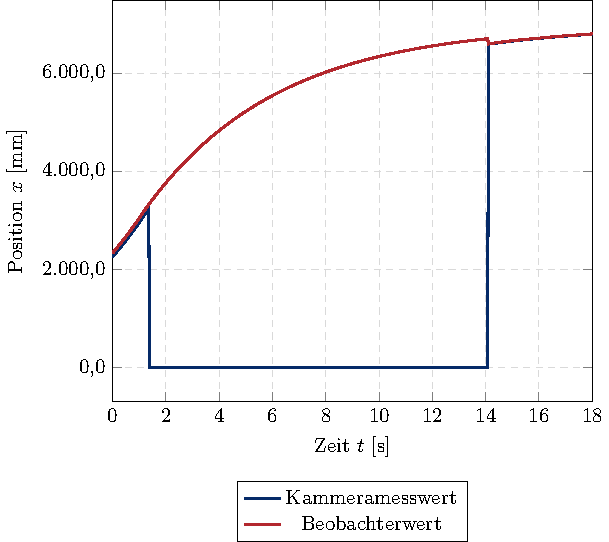
\includegraphics[width=0.8\textwidth]{_Grafiken/Obs_L1_Gesammt.pdf}
    \caption{Beobachter mit direktem Ausgleich Gesammt}
    \label{fig:Obs_L1_Gesammt}
\end{figure}
\begin{figure}[ht]
    \centering
    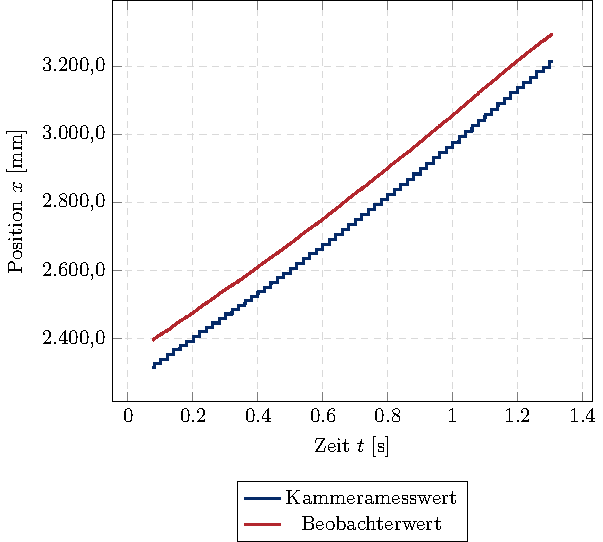
\includegraphics[width=0.8\textwidth]{_Grafiken/Obs_L1_Normalfahrt.pdf}
    \caption{Beobachter mit direktem Ausgleich Normalfahrt}
    \label{fig:Obs_L1_Normalfahrt}
\end{figure}
\begin{figure}[ht]
    \centering
    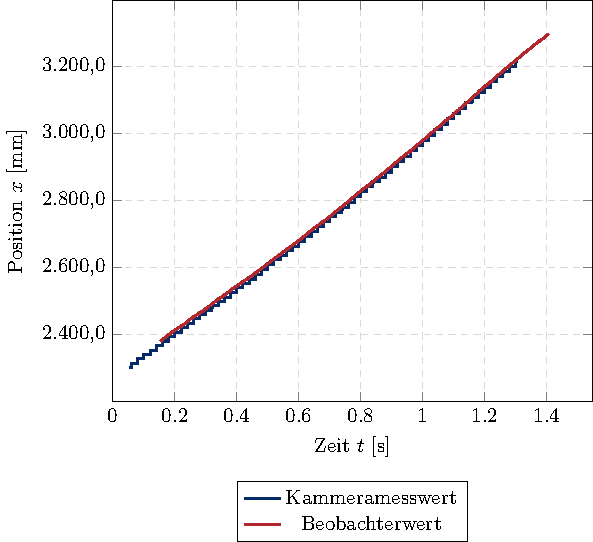
\includegraphics[width=0.8\textwidth]{_Grafiken/Obs_L1_NormalfahrtVerschoben.pdf}
    \caption{Beobachter mit direktem Ausgleich Normalfahrt Verschoben}
    \label{fig:Obs_L1_NormalfahrtVerschoben}
\end{figure}
\begin{figure}[ht]
    \centering
    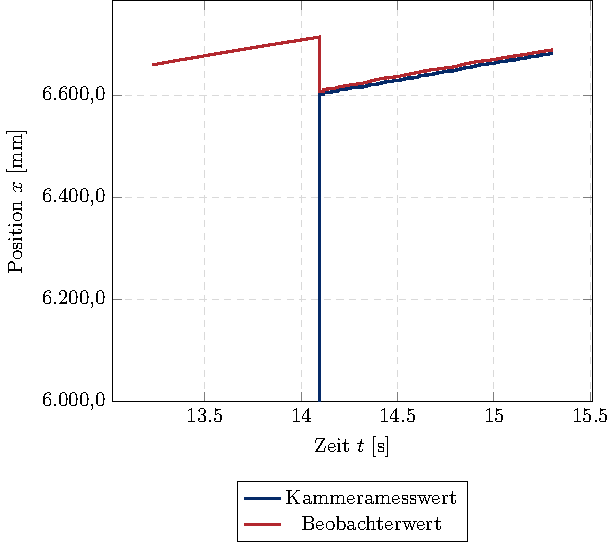
\includegraphics[width=0.8\textwidth]{_Grafiken/Obs_L1_Ausgleich.pdf}
    \caption{Beobachter mit direktem Ausgleich}
    \label{fig:Obs_L1_Ausgleich}
\end{figure}

\begin{figure}[ht]
    \centering
    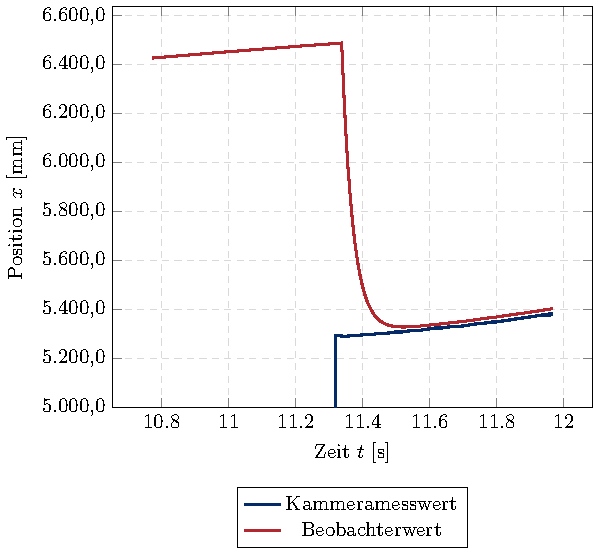
\includegraphics[width=0.8\textwidth]{_Grafiken/Obs_L01_Ausgleich.pdf}
    \caption{Beobachter mit langsamen Ausgleich}
    \label{fig:Obs_L01_Ausgleich}
\end{figure}

\begin{figure}[ht]
    \centering
    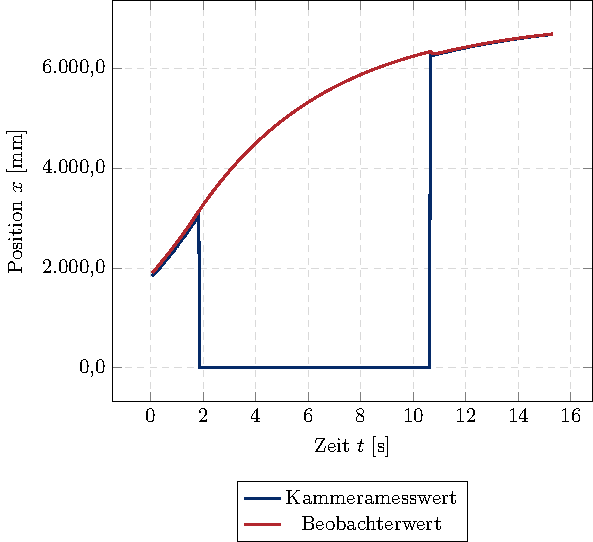
\includegraphics[width=0.8\textwidth]{_Grafiken/Obs_VarGain_Gesammt.pdf}
    \caption{Beobachter mit variablen Gain}
    \label{fig:Obs_VarGain_Gesammt}
\end{figure}
Is von der Idee her ganz nett, aber kein großer Effekt, da die Kamera, wenn Bild Erkannt, immer ähnlichen Fehler aufweißt. Also lieber statischen Wert tunen.